\documentclass[t]{beamer}

\usetheme{CambridgeUS}
\usecolortheme{beaver}
\setbeamertemplate{navigation symbols}{}

\usepackage[utf8]{inputenc}
\usepackage[croatian]{babel}

\usepackage{datetime}
\renewcommand{\dateseparator}{.}
\newcommand{\todayiso}{\twodigit\day \dateseparator \twodigit\month \dateseparator \the \year}
\date{\todayiso}

\usepackage{listings}
\usepackage{graphicx}
\usepackage[export]{adjustbox}
\usepackage{subcaption}
\captionsetup{compatibility=false}
\usepackage{multicol}

\title[NKOSL]{Napredno korištenje operacijskog sustava Linux}
\author[Petar Šegina]{Petar Šegina\\ {\small Nositelj: doc.dr.sc. Stjepan Groš}}
\subtitle{3. Mrežni protokoli}
\institute[FER]{Sveučilište u Zagrebu\\Fakultet elektrotehnike i računarstva}


\begin{document}

{
	\setbeamertemplate{footline}{}
	\begin{frame}
		\maketitle
	\end{frame}
}

\begin{frame}
	\frametitle{Sadržaj}
	\tableofcontents
\end{frame}

\begin{frame}
	\topskip0pt
	\vspace*{\fill}
		\begin{center}
			\Huge{Mrežni protokoli}
		\end{center}
	\vspace*{\fill}
\end{frame}

\begin{frame}{Open Systems Interconnection Reference Model}
    \begin{itemize}
        \item Fizički sloj - Ethernet, USB, ISDN, 802.11, Bluetooth
        \item Podatkovni sloj - Ethernet, ARP, MAC, CSMA/CA 
        \item Mrežni sloj - ICMP, IPsec, IPv4, IPv6, AppleTalk
        \item Transportni sloj - UDP, TCP
        \item Sjednički sloj - SOCKS, SAP, RTP
        \item Prezentacijski sloj - MIME
        \item Aplikacijski sloj - DNS, DHCP, FTP, HTTP, SMTP
    \end{itemize}
\end{frame}

\begin{frame}{Request For Comments}
    \textit{A Request for Comments (RFC), in the context of Internet governance, is a type of publication from the Internet Engineering Task Force (IETF) and the Internet Society (ISOC), the principal technical development and standards-setting bodies for the Internet. (...) RFCs have since become official documents of Internet specifications, communications protocols, procedures, and events.}\footnote{\url{https://en.wikipedia.org/wiki/Request_for_Comments}}
\end{frame}

\section{Osnovni protokoli mrežne komunikacije - UDP i TCP}

\begin{frame}
	\frametitle{UDP i TCP}
	\begin{itemize}
	    \item Transportni protokoli izgrađeni nad IP - Internet Protocol
	    \item Nisu jedini - SCTP, RDP, ...\footnote{\url{https://en.wikipedia.org/wiki/Category:Transport_layer_protocols}}
	    \item User Datagram Protocol
	    \begin{itemize}
	        \item RFC 768 - \url{https://tools.ietf.org/html/rfc768}
	        \item Jednostavan mehanizam slanja poruka među računalima
	    \end{itemize}
	    \item Transmission Control Protocol
	    \begin{itemize}
	        \item RCF 793 - \url{https://tools.ietf.org/html/rfc793}
	        \item Pouzdan, uređen, otporan na greške
	    \end{itemize}
    \end{itemize}
\end{frame}

\begin{frame}{Poslužitelj i klijent}
    \begin{itemize}
        \item netcat
        \begin{itemize}
            \item \textit{(...) a simple Unix utility which reads and writes data across network connections, using TCP or UDP protocol.}\footnote{man netcat}
            \item Poslužitelj
            \begin{itemize}
                \item \texttt{nc -l \{-u|--udp|-t|--tcp\} -p 9998}
                %\item \verb|nc -l \{-u|--udp|-t|--tcp\} -p 9998|
            \end{itemize}
            \item Klijent
            \begin{itemize}
                \item \texttt{nc \{-u|--udp|-t|--tcp\} localhost 9998}
                %\item \verb|nc \{-u|--udp|-t|--tcp\} localhost 9998|
            \end{itemize}
        \end{itemize}
        \item telnet\footnote{\url{https://en.wikipedia.org/wiki/Telnet}}
        \begin{itemize}
            \item teletype network
            \item RFC 15 - \url{https://tools.ietf.org/html/rfc15}
            \item Klijent se može iskoristiti i kao TCP klijent
            \item \texttt{telnet localhost 9998}
        \end{itemize}
    \end{itemize}
\end{frame}

\begin{frame}{TLS - Transport Layer Security}
    \begin{itemize}
        \item Protokoli koje smo naveli su jednostavni - i javno čitljivi
        \item Komunikaciju možemo zaštiti tako da prije pisanja i čitanja podatke kriptiramo
        \begin{itemize}
            \item Sloj \textit{omotač} oko prijenosnih protokola
        \end{itemize}
        \item \url{https://en.wikipedia.org/wiki/Transport_Layer_Security}
        \item TLS v1.2 - RFC 5246 - \url{https://tools.ietf.org/html/rfc5246}
    \end{itemize}
\end{frame}

\section{HTTP(S)}

\begin{frame}{HTTP(S)}
    \begin{itemize}
        \item Hyper Text Transport Protocol (Secure)
        \item TCP 80 i TCP 443
        \item RFC 2616 - \url{https://www.ietf.org/rfc/rfc2616.txt}
        \item Primjer ručnog slanja HTTP zahtjeva
        \begin{itemize}
            \item \texttt{echo "GET / HTTP/1.0\textbackslash{n}\textbackslash{n}" | nc google.com 80}
            %\item \verb|echo "GET / HTTP/1.0\textbackslash{n}\textbackslash{n}" | nc google.com 80
            \begin{itemize}
                \item Nakon nekoliko preusmjeravanja dobivamo Google početnu stranicu
            \end{itemize}
            \item \texttt{echo "GET / HTTP/1.0\textbackslash{n}\textbackslash{n}" | nc google.com 443}
            %\item \verb|echo "GET / HTTP/1.0\textbackslash{n}\textbackslash{n}" | nc google.com 443
            
            \begin{itemize}
                \item Ne dobivamo odgovor - Google očekuje zahtjev kriptiran TLS-om
            \end{itemize}
        \end{itemize}
    \end{itemize}
\end{frame}

\begin{frame}{Slanje TLS zahtjeva}
    \begin{itemize}
        \item Ukoliko radimo ručno sa TCP, moramo sami odraditi i sav posao TLS-a
        \item openssl s\_client - \textit{SSL/TLS client program}\footnote{man openssl s\_client}
        \begin{itemize}
            \item \texttt{echo "GET / HTTP/1.0\textbackslash{n}\textbackslash{n}" | openssl s\_client -ign\_eof\footnote{\url{https://stackoverflow.com/questions/19147280/how-do-you-pipe-echo-into-openssl}} -connect google.com:443}
        \end{itemize}
    \end{itemize}
\end{frame}

\begin{frame}{curl i wget}
    \begin{itemize}
        \item Za rad sa HTTP(S) poslužiteljima možemo koristiti i alate koji su izravno namijenjeni za to
        \item curl
        \begin{itemize}
            \item \textit{is  a tool to transfer data from or to a server, using one of the
               supported protocols (DICT, FILE, FTP, FTPS, GOPHER, HTTP, HTTPS,  IMAP,
               IMAPS,  LDAP,  LDAPS,  POP3,  POP3S,  RTMP, RTSP, SCP, SFTP, SMB, SMBS,
               SMTP, SMTPS, TELNET and TFTP)}\footnote{man curl}
        \end{itemize}
        \item wget
        \begin{itemize}
            \item \textit{\textit{is a free utility for non-interactive download of files from
       the Web.  It supports HTTP, HTTPS, and FTP protocols, as well as
       retrieval through HTTP proxies.}}\footnote{man wget}
            %\item \verb|wget -r --tries=10 http://fly.srk.fer.hr/ -o log\footnote{man wget}|
            \item \texttt{wget -r --tries=10 http://fly.srk.fer.hr/ -o log\footnote{man wget}}
        \end{itemize}
    \end{itemize}
\end{frame}

\begin{frame}
	\topskip0pt
	\vspace*{\fill}
		\begin{center}
			\Huge{Postavljanje vlastitog HTTP poslužitelja na internet}
		\end{center}
	\vspace*{\fill}
\end{frame}

\begin{frame}{GitHub Student Pack}
    \begin{itemize}
        \item \url{https://education.github.com/pack}
        \item Nudi mnogo korisnih alata za razvoj softvera
        \item Uključuje besplatnu .me domenu na Namecheapu
        \item Uključuje \$50 DigitalOcean kredita - dovoljno za 10 mjeseci jednostavnog poslužitelja
        \item Nije jedini izbor, ali je odličan za početi (jer je besplatan)
    \end{itemize}
    
\includegraphics[width=\textwidth,height=80pt,keepaspectratio,right]{studentpack.png}
\end{frame}

\begin{frame}{DigitalOcean}
    \begin{itemize}
        \item \url{https://www.digitalocean.com/}
        \item Infrastructure-As-A-Service provider
        \item Kreiranje Virtual Private Servera unutar 60 sekundi na više lokacija na svijetu
        \item Naplaćivanje po satu\footnote{\url{https://www.digitalocean.com/pricing/}}
    \end{itemize}
    
\includegraphics[width=\textwidth,height=80pt,keepaspectratio,right]{digital_ocean_768.png}
\end{frame}

\begin{frame}{Namecheap}
    \begin{itemize}
        \item \url{https://www.namecheap.com/}
        \item Popularan registar domena
        \item Omogućuje kupovinu i postavljanje mnogo različitih domena
        \item Nudi i besplatnu uslugu DNS posluživanja \footnote{\url{https://www.namecheap.com/domains/freedns/}}
    \end{itemize}
    \vspace*{\fill}
    
\includegraphics[width=80pt,height=80pt,keepaspectratio,right]{namecheap.png}
    \vspace{\fill}
\end{frame}

\begin{frame}{Kreiranje virtualnog poslužitelja na DigitalOcean}
    \begin{itemize}
        \item Kreirati \textit{Droplet}
        
\includegraphics[width=100pt,height=100pt,keepaspectratio,left]{digital_ocean_create.png}
        \item Pričekati minutu
        \item \textit{Droplet} je spreman za korištenje, a lozinka dolazi e-mailom
        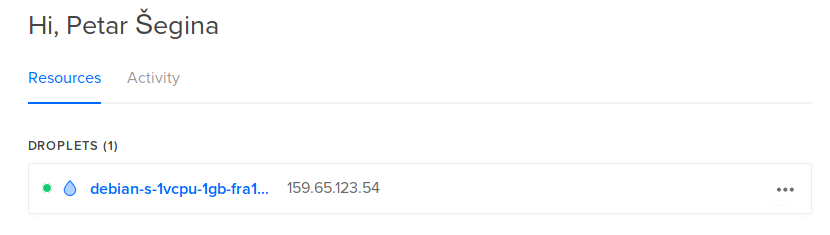
\includegraphics[width=200pt,height=200pt,keepaspectratio,left]{digital_ocean_dashboard.png}
    \end{itemize}
\end{frame}

\section{Upravljanje udaljenim računalom - SSH}

\begin{frame}{Upravljanje udaljenim računalom - SSH}
    \begin{itemize}
        \item Secure Shell protocol
        \item TCP 22
        \item RFC 4253 - \url{https://tools.ietf.org/html/rfc4253}
    \end{itemize}
    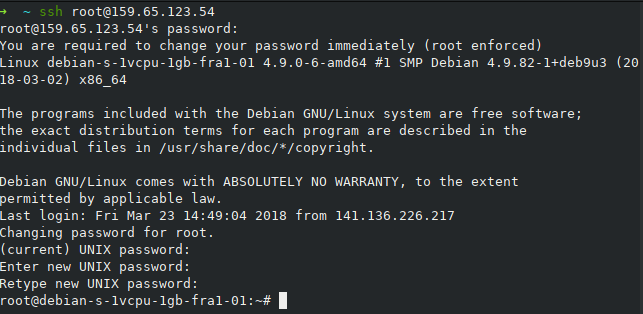
\includegraphics[width=\textwidth,keepaspectratio,center]{ssh.png}
\end{frame}

\begin{frame}{SSH - dodatne funkcionalnosti}
    \begin{itemize}
        \item $\sim$/.ssh\_config\footnote{man ssh\_config}
        \item Autorizacija ključem
        \begin{itemize}
            \item Autorizacija samo lozinkom nije sigurna
            \begin{itemize}
                \item Može se u potpunosti onemogućiti kako bi se smanjila količina bruteforce pokušaja
            \end{itemize}
            \item \url{https://www.digitalocean.com/community/tutorials/how-to-use-ssh-keys-with-digitalocean-droplets}
            \item Poslužitelju se nude svi lokalni ključevi
            \begin{itemize}
                \item Problem za privatnost lokalnog stroja
                \item Dobra ideja namjestiti ssh\_config tako da poslužiteljima nudi lokalni ključ samo ako je tako deklarirano
            \end{itemize}
        \end{itemize}
        \item Port forwarding - \url{https://blog.trackets.com/2014/05/17/ssh-tunnel-local-and-remote-port-forwarding-explained-with-examples.html}
    \end{itemize}
\end{frame}

\begin{frame}[fragile]{SSH - izvršavanje skripti}
    \begin{itemize}
        \item SSH možemo iskoristiti i kako bi izvršili skripte na udaljenom poslužitelju
        \begin{verbatim}
ssh root@159.65.123.54 << HERE
    hostname;
    date;
HERE
        \end{verbatim}
    \end{itemize}
\end{frame}

\begin{frame}{SSH - poslužitelj}
    \begin{itemize}
        \item Na poslužitelj se možemo spojiti putem SSH jer se na njemu izvršava SSH poslužitelj
        \item Primjerice, sshd - OpenSSH SSH daemon\footnote{man sshd}
    \end{itemize}
\end{frame}

\begin{frame}{Poslužitelj nginx}
    \begin{itemize}
        \item \textit{a free, open-source, high-performance HTTP server and reverse proxy}\footnote{\url{https://www.nginx.com/resources/wiki/}}
        \item Jednostavan za uporabu i veoma brz
        \item \texttt{apt update \&\& apt install nginx}
        \item nginx sada poslužuje HTML stranu sa \textit{/usr/share/nginx/html/index.html}
    \end{itemize}
\end{frame}

\begin{frame}{Let's Encrypt}
    \begin{itemize}
        \item Naša strana je dostupna na internetu, ali nije zaštićena
        \item Da bi komunikacija s klijentima bila sigurna, potrebno ju je zaštiti TLS-om
        \item Potrebno je dobiti certificat od nekog \textit{Certificate Authorityja} kojem preglednici vjeruju
        \item Najjednostavnije (i besplatno) rješenje - Let's Encrypt\footnote{\url{https://letsencrypt.org/}}
        \begin{itemize}
            \item Jednostavan za postaviti uz nginx\footnote{\url{https://www.digitalocean.com/community/tutorials/how-to-secure-nginx-with-let-s-encrypt-on-ubuntu-16-04}}
        \end{itemize}
    \end{itemize}
\end{frame}

\begin{frame}
	\topskip0pt
	\vspace*{\fill}
		\begin{center}
			\Huge{Imamo svoj kutak interneta!} \\
			\small{(Ali nitko neće pamtiti našu IP adresu)}
		\end{center}
	\vspace*{\fill}
\end{frame}

\section{Imenovanje računala - DNS}

\begin{frame}{Imenovanje računala - DNS}
    \begin{itemize}
        \item Domain Name System
        \item UDP 53
        \item RFC 1035 - \url{https://www.ietf.org/rfc/rfc1035.txt}
        \item Pohranjuje podatke o domeni
        \begin{itemize}
            \item Koja je adresa poslužitelja za domenu? (A i AAAA)
            \item Koji je mail poslužitelj za ovu domenu? (MX)
            \item Pokazuje li ova domena na neku drugu? (CNAME)
            \item Proizvoljan tekst vezan uz ovu domenu? (TXT)
            \item i drugi\footnote{\url{https://en.wikipedia.org/wiki/List_of_DNS_record_types}}
        \end{itemize}
    \end{itemize}
\end{frame}

\begin{frame}[fragile]{DNS upiti - alat dig}
    \begin{itemize}
        \item \textit{Domain Information Grouper}\footnote{\url{https://ns1.com/articles/decoding-dig-output}}
        \item \textit{DNS lookup utility}\footnote{man dig}
        \item {\footnotesize \begin{verbatim}
dig @8.8.8.8 +noall +answer ANY fer.hr
fer.hr.			3422	IN	A	161.53.72.119
fer.hr.			3422	IN	SOA	labs5.fer.hr. postmaster.labs5.fer.hr. 2018031301 28800 7200 1209600 3600
fer.hr.			422	IN	MX	1 fer-hr.mail.protection.outlook.com.
fer.hr.			3422	IN	TXT	"tWfeXfT/8dO+7Lpa5REWh3pASQErEh8gLqYU4hQ6u4VdJTY7tlc3JivomJiwOIs5KUDOmcgQUs3mtcbG+rBhnQ=="
fer.hr.			3422	IN	NS	labs5.fer.hr.
fer.hr.			3422	IN	TXT	"MS=34689B116A78E433D9BB3A222006AFE3F0010A5B"
fer.hr.			3422	IN	NS	sysdns.carnet.hr.
        \end{verbatim}}
        \item DiG HOWTO - \url{https://www.madboa.com/geek/dig/}
    \end{itemize}
\end{frame}

\begin{frame}[fragile]{Može li i jednostavnije?}
    \begin{itemize}
        \item \textit{/etc/hosts}
        \begin{itemize}
            \item Jednostavno mapiranje IP adrese na hostname\footnote{man hosts}
            \item Zgodan način za blokiranje određenih poslužitelja
        \end{itemize}
    \end{itemize}
\end{frame}

\begin{frame}
	\topskip0pt
	\vspace*{\fill}
		\begin{center}
			\Huge{Kako postaviti svoju domenu?}
		\end{center}
	\vspace*{\fill}
\end{frame}

\begin{frame}{Namecheap - postavljanje DNS upisa}
    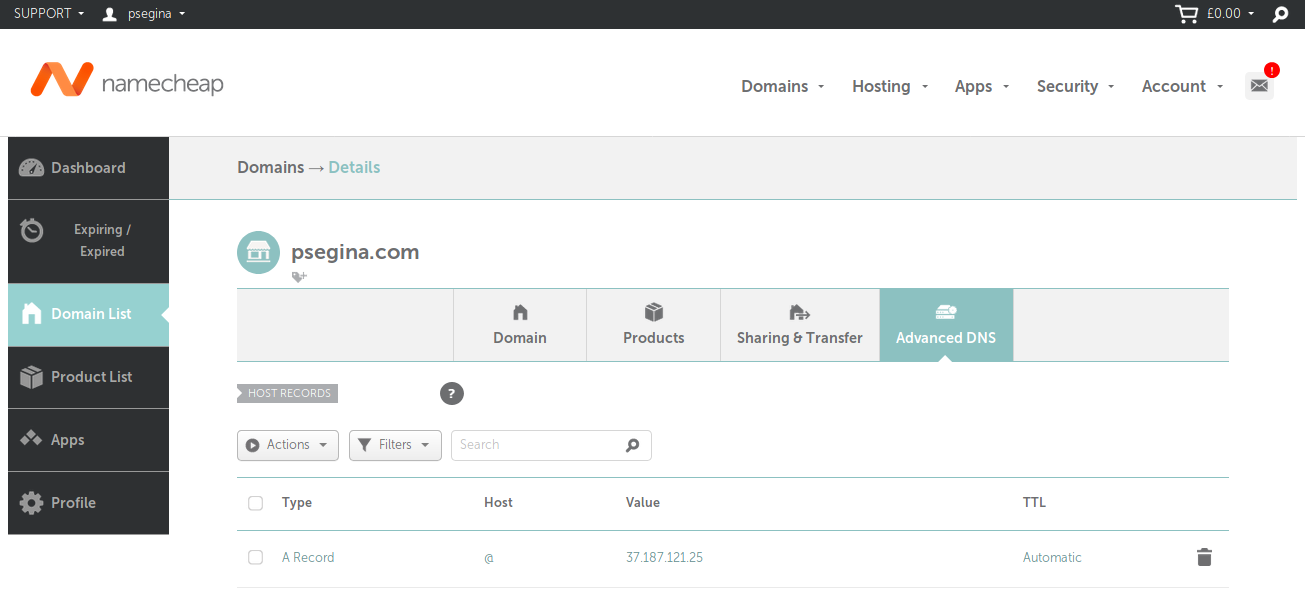
\includegraphics[width=\textwidth,keepaspectratio,center]{namecheap-dns.png}
\end{frame}

\section{Upravljanje datotekama - SCP, FTP, FTPS, SFTP}

\begin{frame}{Upravljanje datotekama - SCP, FTP, FTPS, SFTP}
    \begin{itemize}
        \item Preko SSH možemo direktno uređivati datoteke na poslužitelju
        \begin{itemize}
            \item No to nije praktično
        \end{itemize}
        \item Za jednostavnije upravljanje datotekama na poslužitelju možemo koristiti neki od specijaliziranih protokola
        \begin{itemize}
            \item SCP
            \begin{itemize}
                \item \textit{secure copy (remote file copy program)}\footnote{man scp}
                \item Dolazi sa SSH - RFC 4251 - \url{https://tools.ietf.org/html/rfc4251}
                \item Način korištenja sličan cp
                \item \texttt{
                    scp lokalna\_datoteka.bin user@host:/usr/share/nginx/html/
                }
            \end{itemize}
            \item FTP(S)
            \begin{itemize}
                \item RFC 959 - \url{https://tools.ietf.org/html/rfc959.html}
                \item Potrebno podesiti FTP daemon na poslužitelju
                \item Primjerice - vsftpd\footnote{\url{https://security.appspot.com/vsftpd.html}}\footnote{\url{https://www.digitalocean.com/community/tutorials/how-to-set-up-vsftpd-for-a-user-s-directory-on-ubuntu-16-04}}
            \end{itemize}
        \end{itemize}
    \end{itemize}
\end{frame}

\begin{frame}{Upravljanje datotekama - SCP, FTP, FTPS, SFTP}
    \begin{itemize}
        \item Za jednostavnije upravljanje datotekama na poslužitelju možemo koristiti neki od specijaliziranih protokola
        \begin{itemize}
            \item SFTP
            \begin{itemize}
                \item \textit{SSH File Transfer Protocol}\footnote{\url{https://en.wikipedia.org/wiki/SSH_File_Transfer_Protocol}}
                \item Proširenje protokola SSH
                \item Za razliku od SCP nudi i druge operacije nad datotečnim sustavom osim kopiranja
            \end{itemize}
        \end{itemize}
    \end{itemize}
\end{frame}


\section{Dinamično generirani sadržaj - (F)CGI}

\begin{frame}{Dinamično generirani sadržaj - (F)CGI}
    \begin{itemize}
        \item Možemo posluživati statičke datoteke, no kako posluživati dinamičan sadržaj?
        \item Common Gateway Interface
        \begin{itemize}
            \item RFC 3875 - \url{https://tools.ietf.org/html/rfc3875}
            \item Ne moramo svaki puta nanovo implementirati zaduženja HTTP poslužitelja
            \item HTTP poslužitelj primi zahtjev
            \item Pokrene naš program i na njegov standardni ulaz i okolinu pošalje primljene podatke
            \item Ono što program ispiše na svoj standardni izlaz pošalje klijentu
            \item Nedostatak - za svaki zahtjev stvara se novi proces
            \begin{itemize}
                \item Proširenje - Fast CGI\footnote{\url{http://www.mit.edu/~yandros/doc/specs/fcgi-spec.html}}
            \end{itemize}
        \end{itemize}
        \item \url{https://www.howtoforge.com/serving-cgi-scripts-with-nginx-on-debian-squeeze-ubuntu-11.04-p3}
    \end{itemize}
\end{frame}

\section{e-mail, kalendar i kontakti}

\begin{frame}{e-mail, kalendar i kontakti}
    \begin{itemize}
        \item e-mail
        \begin{itemize}
            \item Slanje - \textit{Simple Mail Transfer Protocol}\footnote{\url{https://tools.ietf.org/html/rfc5321}}
            \item Pristup sandučiću - \textit{Internet Message Access Protocol}\footnote{\url{https://tools.ietf.org/html/rfc1730}} i \textit{Post Office Protocol}\footnote{\url{https://tools.ietf.org/html/rfc1081}}
            \item Protokoli ne koriste TLS \textit{po defaultu} - varijante SMTPS, IMAPS, POP3S, StartTLS\footnote{\url{https://en.wikipedia.org/wiki/Opportunistic_TLS}}
        \end{itemize}
    \end{itemize}
\end{frame}

\begin{frame}{e-mail, kalendar i kontakti}
    \begin{itemize}
        \item WebDAV
        \begin{itemize}
            \item \textit{Web Distributed Authoring and Versioning}\footnote{https://en.wikipedia.org/wiki/WebDAV}
            \item RFC 4918 - \url{https://tools.ietf.org/html/rfc4918}
            \item Proširenje HTTP-a koje omogućuje upravljanje dokumentima na poslužitelju
            \item CardDAV
            \begin{itemize}
                \item \textit{vCard Extensions to WebDAV}\footnote{\url{https://en.wikipedia.org/wiki/CardDAV}}
                \item RFC 6352 - \url{https://tools.ietf.org/html/rfc6352}
            \end{itemize}
            \item CalDAV
            \begin{itemize}
                \item \textit{Calendaring Extensions to WebDAV}\footnote{\url{https://en.wikipedia.org/wiki/CalDAV}}
                \item RFC 4791 - \url{https://tools.ietf.org/html/rfc4791}
            \end{itemize}
        \end{itemize}
    \end{itemize}
\end{frame}

\section{Vrijeme - NTP}

\begin{frame}{Vrijeme - NTP}
    \begin{itemize}
        \item Svako računalo ima svoj sat
        \item Satove među računalima potrebno je sinhronizirati
        \item \textit{Network Time Protocol}\footnote{\url{https://en.wikipedia.org/wiki/Network_Time_Protocol}}
        \begin{itemize}
            \item RFC 958 - \url{https://tools.ietf.org/html/rfc958}
        \end{itemize}
        \item Sinkronizacija pomoću lokalnih servisa
        \begin{itemize}
            \item ntpd\footnote{\url{https://en.wikipedia.org/wiki/Ntpd}}
            \item systemd-timesyncd\footnote{\url{https://wiki.archlinux.org/index.php/systemd-timesyncd}}
        \end{itemize}
        \item Važno je imati ispravno podešeno vrijeme, u suprotnom neke usluge mogu prestati ispravno raditi
        \begin{itemize}
            \item TLS
            \item DNS
            \item e-mail
        \end{itemize}
    \end{itemize}
\end{frame}

\section{VPN}

\begin{frame}{VPN}
    \begin{itemize}
        \item \textit{Virtual Private Network}
        \item Omogućava da se ponašamo kao da smo dio neke druge privatne mreže
        \item Možemo pristupati resursima samo unutar mreže
        \item Možemo pristupati vanjskim resursima šaljući zahtjeve iz te mreže
        \item Podiže razinu sigurnosti i privatnosti mrežnog pristupa
        \item OpenVPN - \url{https://openvpn.net/}
        \item \url{https://www.digitalocean.com/community/tutorials/how-to-set-up-an-openvpn-server-on-ubuntu-16-04}
    \end{itemize}
\end{frame}

\section*{}

\begin{frame}{Kamo dalje?}
    \begin{itemize}
        \item Na FER-u
        \begin{itemize}
            \item Komunikacijske mreže\footnote{\url{https://www.fer.unizg.hr/predmet/kommre}}
            \item Mrežno programiranje \footnote{\url{https://www.fer.unizg.hr/predmet/mrepro}}
            \item Raspodijeljeni sustavi\footnote{\url{https://www.fer.unizg.hr/predmet/rassus}}
            \item Osnove izrade PHP aplikacija \footnote{\url{https://www.fer.unizg.hr/predmet/oipa}}
            \item NKOSL - o mrežama i uslugama pričat ćemo još
        \end{itemize}
        \item Beej's Guide to Network Programming\footnote{\url{https://beej.us/guide/bgnet/}}
        \item Uz znanje dobiveno danas, pokušajte sami postaviti svoju web stranicu
        \begin{itemize}
            \item Shameless plug - \url{https://psegina.com}
            \item Obavezno nam pošaljite link na 
            \href{mailto:nkosl@kset.org}{nkosl@kset.org}
        \end{itemize}
    \end{itemize}
\end{frame}

\begin{frame}{Literatura}
\url{https://en.wikipedia.org/wiki/Request_for_Comments}\\
\url{https://en.wikipedia.org/wiki/Category:Transport_layer_protocols}\\
\url{https://tools.ietf.org/html/rfc768}\\
\url{https://tools.ietf.org/html/rfc793}\\
\url{https://en.wikipedia.org/wiki/Telnet}\\
\url{https://tools.ietf.org/html/rfc15}\\
\url{https://en.wikipedia.org/wiki/Transport_Layer_Security}\\
\url{https://tools.ietf.org/html/rfc5246}\\
\url{https://www.ietf.org/rfc/rfc2616.txt}\\
\url{https://stackoverflow.com/questions/19147280/how-do-you-pipe-echo-into-openssl}
\end{frame}

\begin{frame}{Literatura}
\url{https://education.github.com/pack}\\
\url{https://www.digitalocean.com/}\\
\url{https://www.digitalocean.com/pricing/}\\
\url{https://www.namecheap.com/}\\
\url{https://www.namecheap.com/domains/freedns/}\\
\url{https://tools.ietf.org/html/rfc4253}\\
\url{https://www.digitalocean.com/community/tutorials/how-to-use-ssh-keys-with-digitalocean-droplets}\\
\url{https://blog.trackets.com/2014/05/17/ssh-tunnel-local-and-remote-port-forwarding-explained-with-examples.html}\\
\url{https://www.nginx.com/resources/wiki/}\\
\url{https://letsencrypt.org/}\\
\end{frame}

\begin{frame}{Literatura}
\url{https://www.digitalocean.com/community/tutorials/how-to-secure-nginx-with-let-s-encrypt-on-ubuntu-16-04}\\
\url{https://www.ietf.org/rfc/rfc1035.txt}\\
\url{https://en.wikipedia.org/wiki/List_of_DNS_record_types}\\
\url{https://ns1.com/articles/decoding-dig-output}\\
\url{https://www.madboa.com/geek/dig/}\\
\url{https://tools.ietf.org/html/rfc4251}\\
\url{https://tools.ietf.org/html/rfc959.html}\\
\url{https://www.digitalocean.com/community/tutorials/how-to-set-up-vsftpd-for-a-user-s-directory-on-ubuntu-16-04}\\
\url{https://en.wikipedia.org/wiki/SSH_File_Transfer_Protocol}\\
\url{https://tools.ietf.org/html/rfc3875}\\
\end{frame}

\begin{frame}{Literatura}
\url{http://www.mit.edu/~yandros/doc/specs/fcgi-spec.html}\\
\url{https://www.howtoforge.com/serving-cgi-scripts-with-nginx-on-debian-squeeze-ubuntu-11.04-p3}\\
\url{https://tools.ietf.org/html/rfc5321}\\
\url{https://tools.ietf.org/html/rfc1081}\\
\url{https://en.wikipedia.org/wiki/Opportunistic_TLS}\\
\url{https://tools.ietf.org/html/rfc4918}\\
\url{https://en.wikipedia.org/wiki/CardDAV}\\
\url{https://tools.ietf.org/html/rfc6352}\\
\url{https://en.wikipedia.org/wiki/CalDAV}\\
\url{https://tools.ietf.org/html/rfc4791}\\
\end{frame}

\begin{frame}{Literatura}
\url{https://en.wikipedia.org/wiki/Network_Time_Protocol}\\
\url{https://tools.ietf.org/html/rfc958}\\
\url{https://en.wikipedia.org/wiki/Ntpd}\\
\url{https://wiki.archlinux.org/index.php/systemd-timesyncd}\\
\url{https://openvpn.net/}\\
\url{https://www.digitalocean.com/community/tutorials/how-to-set-up-an-openvpn-server-on-ubuntu-16-04}\\
\url{https://beej.us/guide/bgnet/}\\
\end{frame}

\end{document}
